\documentclass{ctexart}
\usepackage{amsmath}
\usepackage{amssymb}
\usepackage{graphicx}
\usepackage{gbt7714}
\usepackage{wrapfig}
\ctexset{
    % 修改 section。
    section={   
        name={,、},
        number={\chinese{section}}
    }
}

\title{研究弦线上的驻波现象}
\author{陆知辰-10225301456}
\date{\today}
\graphicspath{{figure/}}

\begin{document}

\begin{titlepage}
  \centering
  % 插入图片
  
\includegraphics[width=0.5\textwidth]{ecnu.png}
  
  % 空行用于调整标题位置
  \vspace*{\baselineskip}
  
  % 标题
  \Huge\textbf{物\quad 理\quad 实\quad 验 \quad (二)}
  % 空行用于调整标题和其他信息之间的间距
  \vspace*{0.3\baselineskip}
  
  % 具体实验名称
  \huge 研究弦线上的驻波现象
  
  % 空行用于调整时间和其他信息之间的间距
  \vspace*{2\baselineskip}
  
  % 时间
  \large 时间:\today
  
  % 空行用于调整时间和其他信息之间的间距
  \vspace*{\baselineskip}
  
  % 创作人
  \large 创作人:陆知辰
  
  % 空行用于调整创作人和学号之间的间距
  \vspace*{\baselineskip}
  
  % 学号
  \large 学号:10225301478
  
\end{titlepage}
\newpage
\tableofcontents
\newpage
\section{实验摘要}
  \subsection{实验概要}
  驻波是由两列传播方向相反、振幅和频率都相等,且相位差恒定的简写波叠加而成的。

  \subsection{实验目的}
  1.\quad 观察弦线上的驻波现象。

  2.\quad 研究弦线张力、振动频率、振幅三者对驻波形成的影响。
  
  3.\quad 学会如何从驻波理论出发,指定验证驻波波长和拉力、频率关系的实验方案。

\section{实验原理}
\begin{figure}[b]
  \centering
  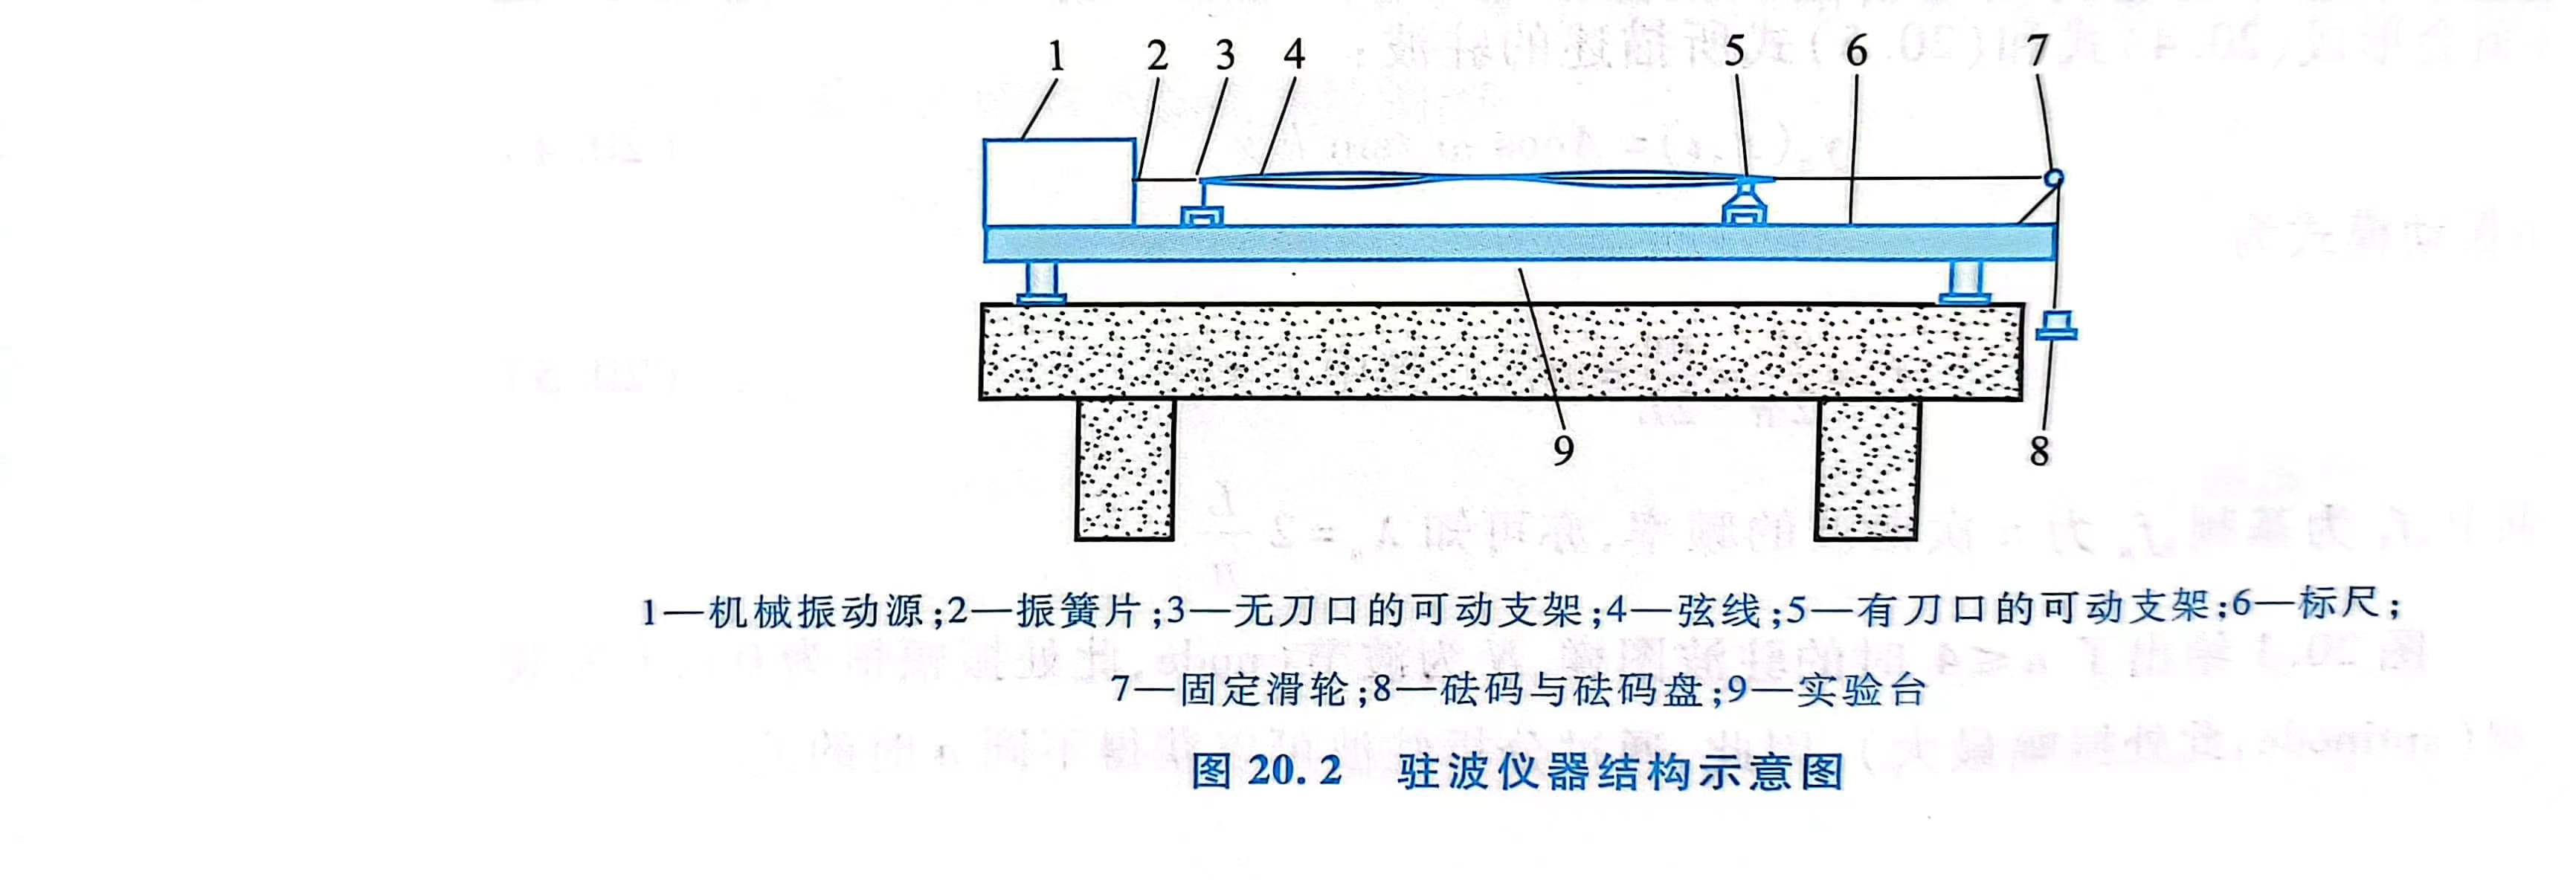
\includegraphics[height=0.3\textwidth,width=1\textwidth]{yuanli1.jpg}
  \caption{实验原理辅助用图}\label{figureyuanli1}
\end{figure}
实验中使用的器材如图\ref{figureyuanli1}。实验中使用该装置获得拉紧的弦线,通过振动弦线产生驻波。
金属弦线一端固定在振动源,另一端固定一个砝码。砝码能够用来使金属弦线拉紧。
同时由于刀口的存在,所以弦线无法振动,所以振动在这个位置被反射,由此形成了从右往左的波和
从左往右的反射波。在这样的条件下也能产生驻波在弦线上。

实验中将最靠近振动端的波节作为测量$L$的起始点,该点到有刀口的可动支架的距离$L$为半波长的整数倍
\begin{equation}
  L=n \frac{\lambda}{2}
\end{equation}

根据对于简谐振动的已学知识,实验中在一根拉紧的弦线上传播的机械振动横波可以被描述为
\begin{equation}\label{jixiezhendonghengbo}
  y\(x \, t\)=A\sin \( \omega t \pm kx\)
\end{equation}
在式\ref{jixiezhendonghengbo}中$y$是弦线在$x$处在$t$时刻的位移。$A$为振幅,$\omega$是振动的角频率,
$k$是角波数。对于式\ref{jixiezhendonghengbo}中出现的对象同时还应该满足波动方程
\begin{equation}\label{bodongfangcheng}
  \frac{\partial ^{2} y\(x,t\)}{\partial x^{2}} = \frac{1}{v^{2}} \frac{\partial ^{2} y\(x,t\)}{\partial t^{2}}

  \mbox{其中} v^{2} = \frac{\omega ^{2}}{k^{2}}
\end{equation}

当开始振动弦线的时候,振动源会给弦线力的作用,这里假设张力为$F_{T}$,弦线的密度为$\rho _{2}$,则
可以得到弦线上沿弦线传播的横波的速度为
\begin{equation}\label{bosufangcheng}
  v=\sqrt[2]{\frac{F_{T}}{\rho _{2}}}
\end{equation}

而弦线两端固定,且长度为$L$,所以同时还需要满足振动的边界条件$y(0)=y(L)=0$,由于两端的端点是固定的,所以
传播的时候产生的波和反射波最终会相互叠加在弦线上形成驻波。驻波应该满足以下条件:
\begin{equation}\label{zhubofangcheng}
  y_{n}\(x,t\)=A\cos \omega _{n} t \sin k_{n} x
\end{equation}

同时还应该满足
\begin{equation}\label{zhendongmoshi}
  f_{n}=\frac{\omega _{n}}{2\pi}=\frac{nv}{2L}=nf_{1}\mbox{,其中}f_{1}=\frac{v}{2L}
\end{equation}
在式\ref{zhendongmoshi}中,$f_{1}$为基频,$f_{n}$为$n$次谐波的频率,由此可以得到
波长的表达形式为$\lambda_{n}=2\frac{L}{n}$

\begin{figure}[b]
  \centering
  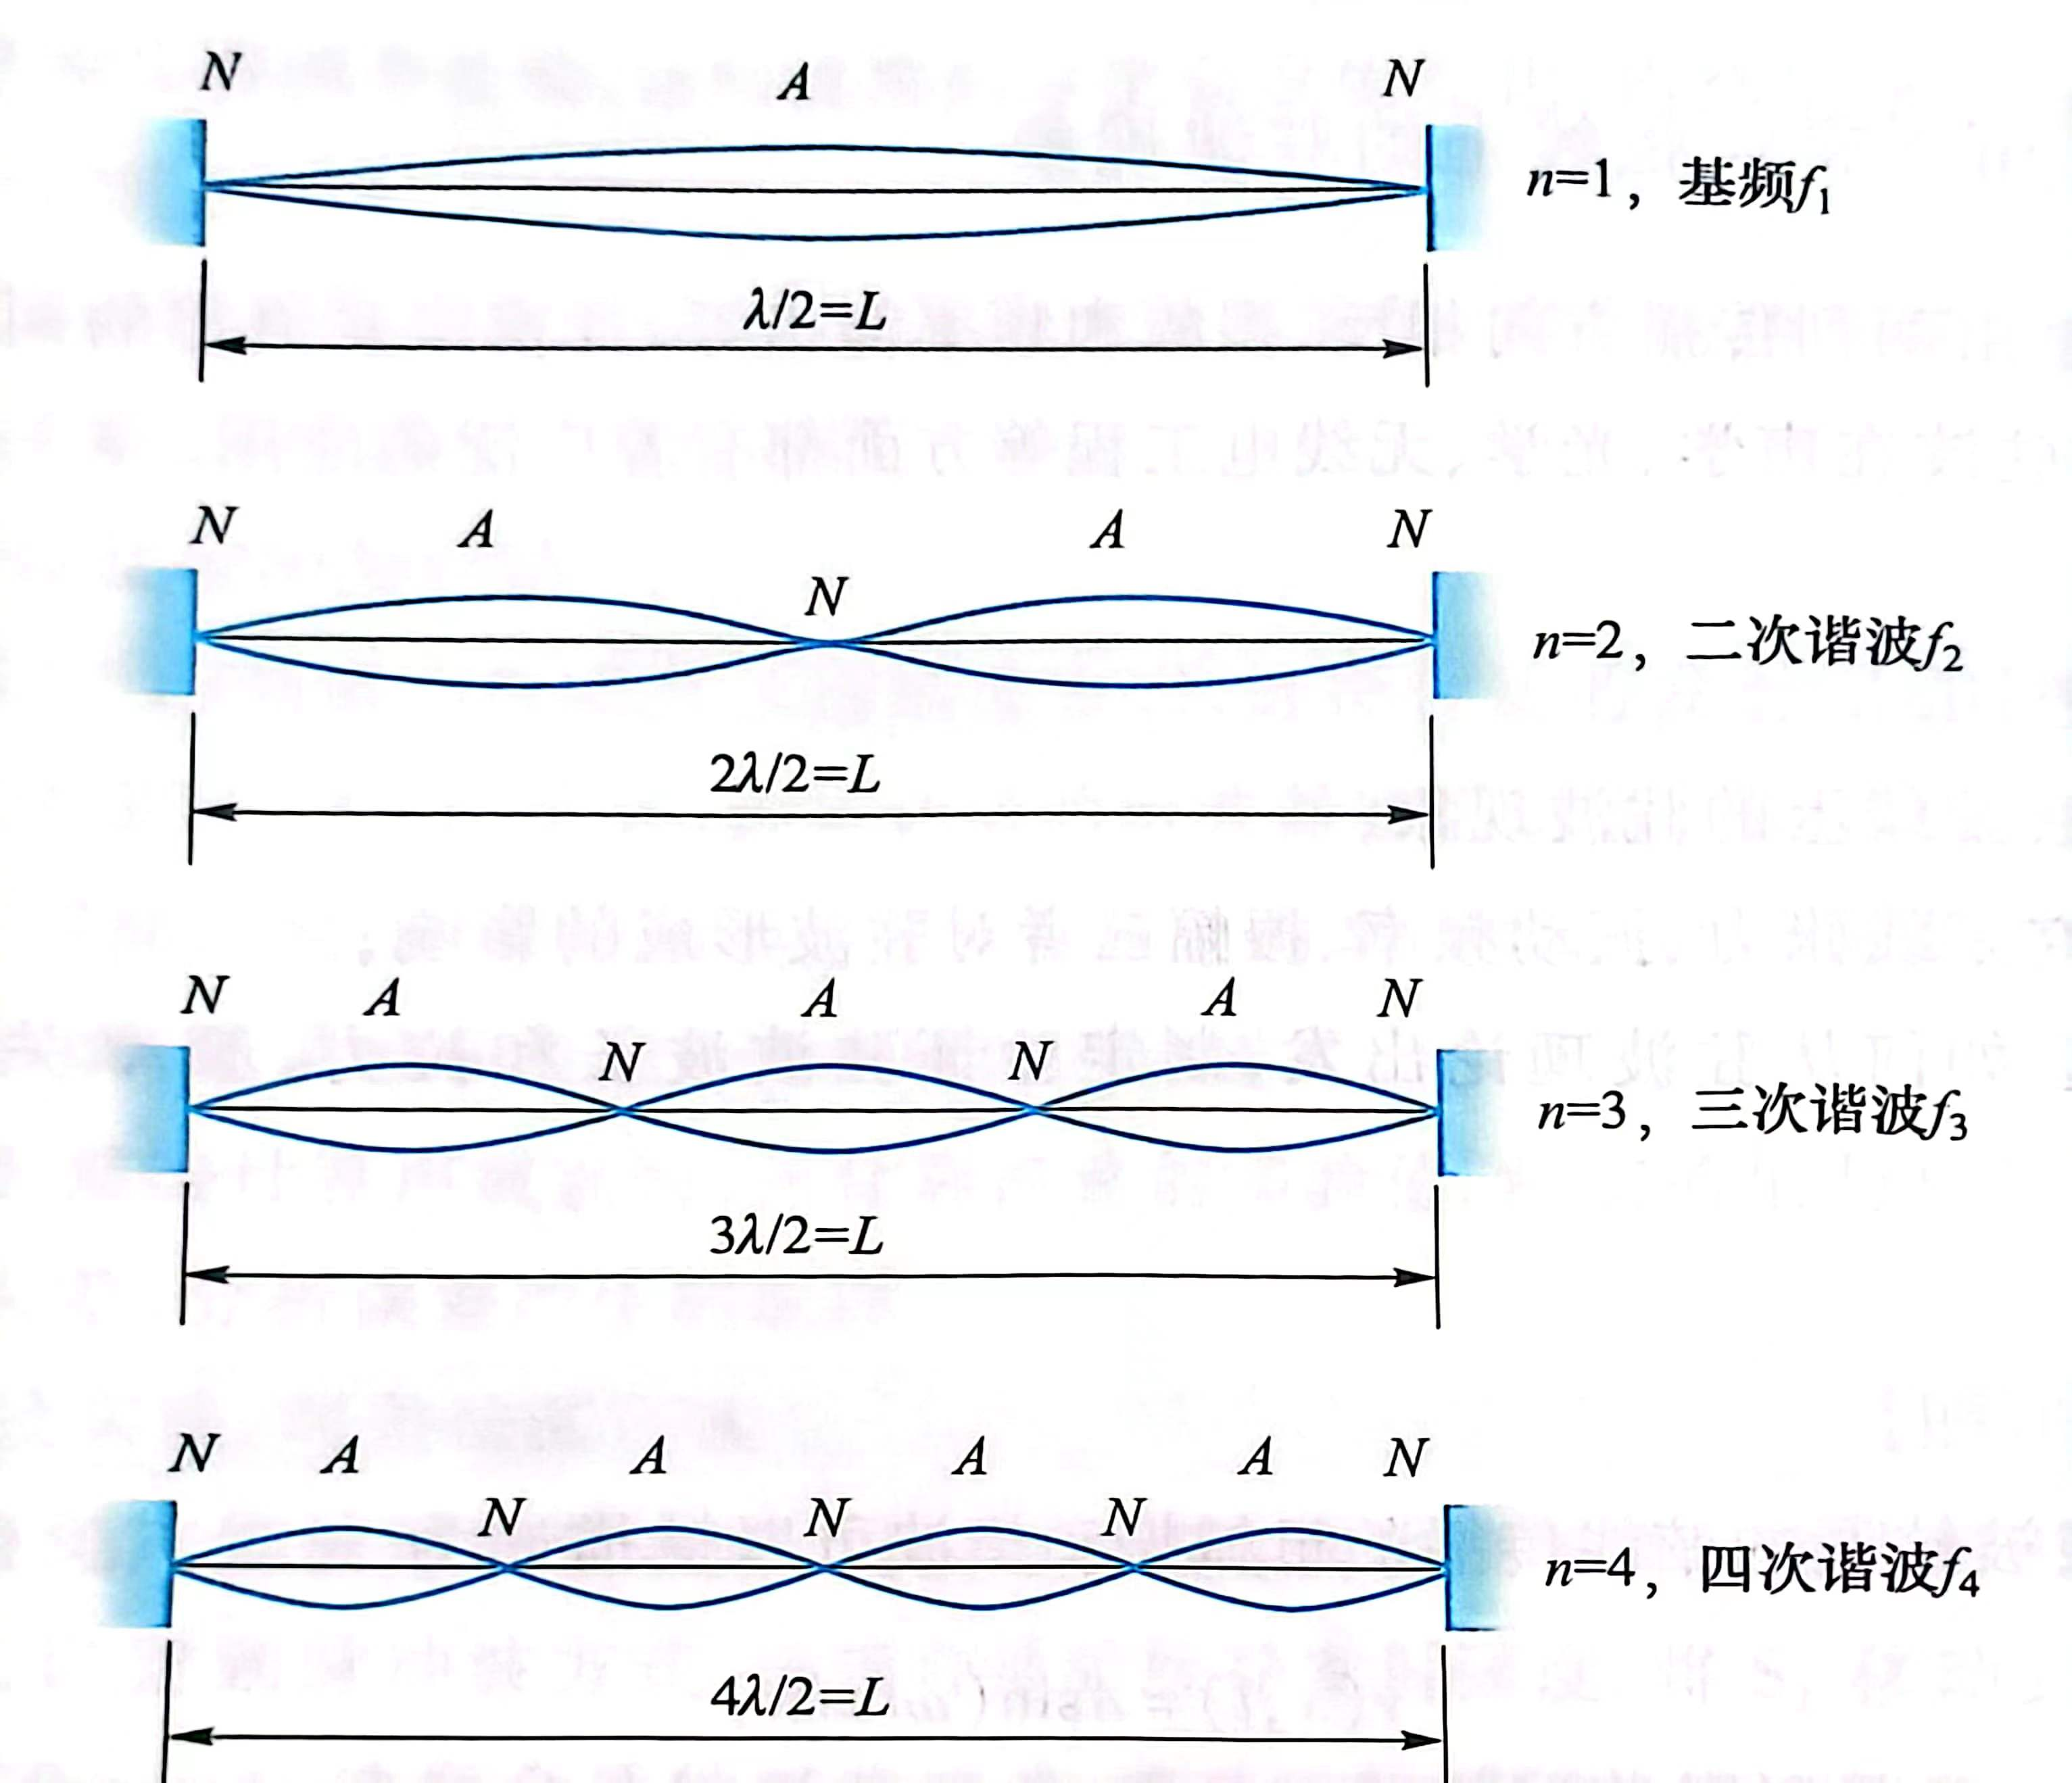
\includegraphics[height=0.3\textwidth,width=1\textwidth]{zhuboyanshi.jpg}
  \caption{光电门与滑块位置关系示意图}\label{zhuboyanshi}
\end{figure}

图\ref{zhuboyanshi}演示了在当$n\leq 4$的时候驻波的示意图像。其中$N$为波节。波节就是
振幅恒等于0的位置,$A$为波腹。波腹就是振幅最大的位置。由此图像可以直接通过观察得出$\lambda$
以及$f_{n}$表达。

根据之前得到的式\ref{bosufangcheng}能够进一步推导得出波长$\lambda$的表达形式为
\begin{equation}\label{bochangfangcheng}
  \lambda = \frac{v}{f} =\frac{1}{f}\sqrt[2]{\frac{F_{T}}{\mu}}
\end{equation}
再对式\ref{bochangfangcheng}两边取对数,就可以进一步得到
\begin{equation}\label{bochangduishufangcheng}
  \ln \lambda = \frac{1}{2} \ln F_{T}-\frac{1}{2} \ln \mu - \ln f
\end{equation}
通过式\ref{bochangduishufangcheng}可以通过实验得到数据并对数据进行
图像化处理后得到$\lambda - T$以及$\lambda -f$的图像和拟合方程。
由此验证弦线中$\lambda - T$以及$\lambda -f$的特性。

\section{实验装置器材介绍}
频率可调节的机械振动源、实验台、固定滑轮、刻度尺、不同粗细的弦线若干、
砝码盘、砝码若干、电子天平、频闪灯

\section{实验内容及实验步骤}
  \subsection{实验准备}
  实验前测量砝码的质量并记录,多次测量取平均值。并正确组装装置,保证实验中刀口能固定弦线,
  能产生反射波。
  \subsection{预实验}
  在装置组装完成后打开各项设备的开关,进行预实验。观察不同张力下的半波长出现的数量。之后调节
  机械振动源改变波动频率,观察不同波动频率下半波长出现的数量。之后调节刀口位置,左右滑动刀口的
  滑轮,观察振幅改变情况以及半波长出现的数量。

  通过预实验得到定性的结果,并定性描述弦线张力、波动频率、振幅三者对驻波形成的影响。
  \subsection{}

  \subsection{}
    \subsubsection{}
    \subsubsection{}

  \subsection{}
\newpage

\section{实验原始数据}
\begin{figure}[h]
  \centering
  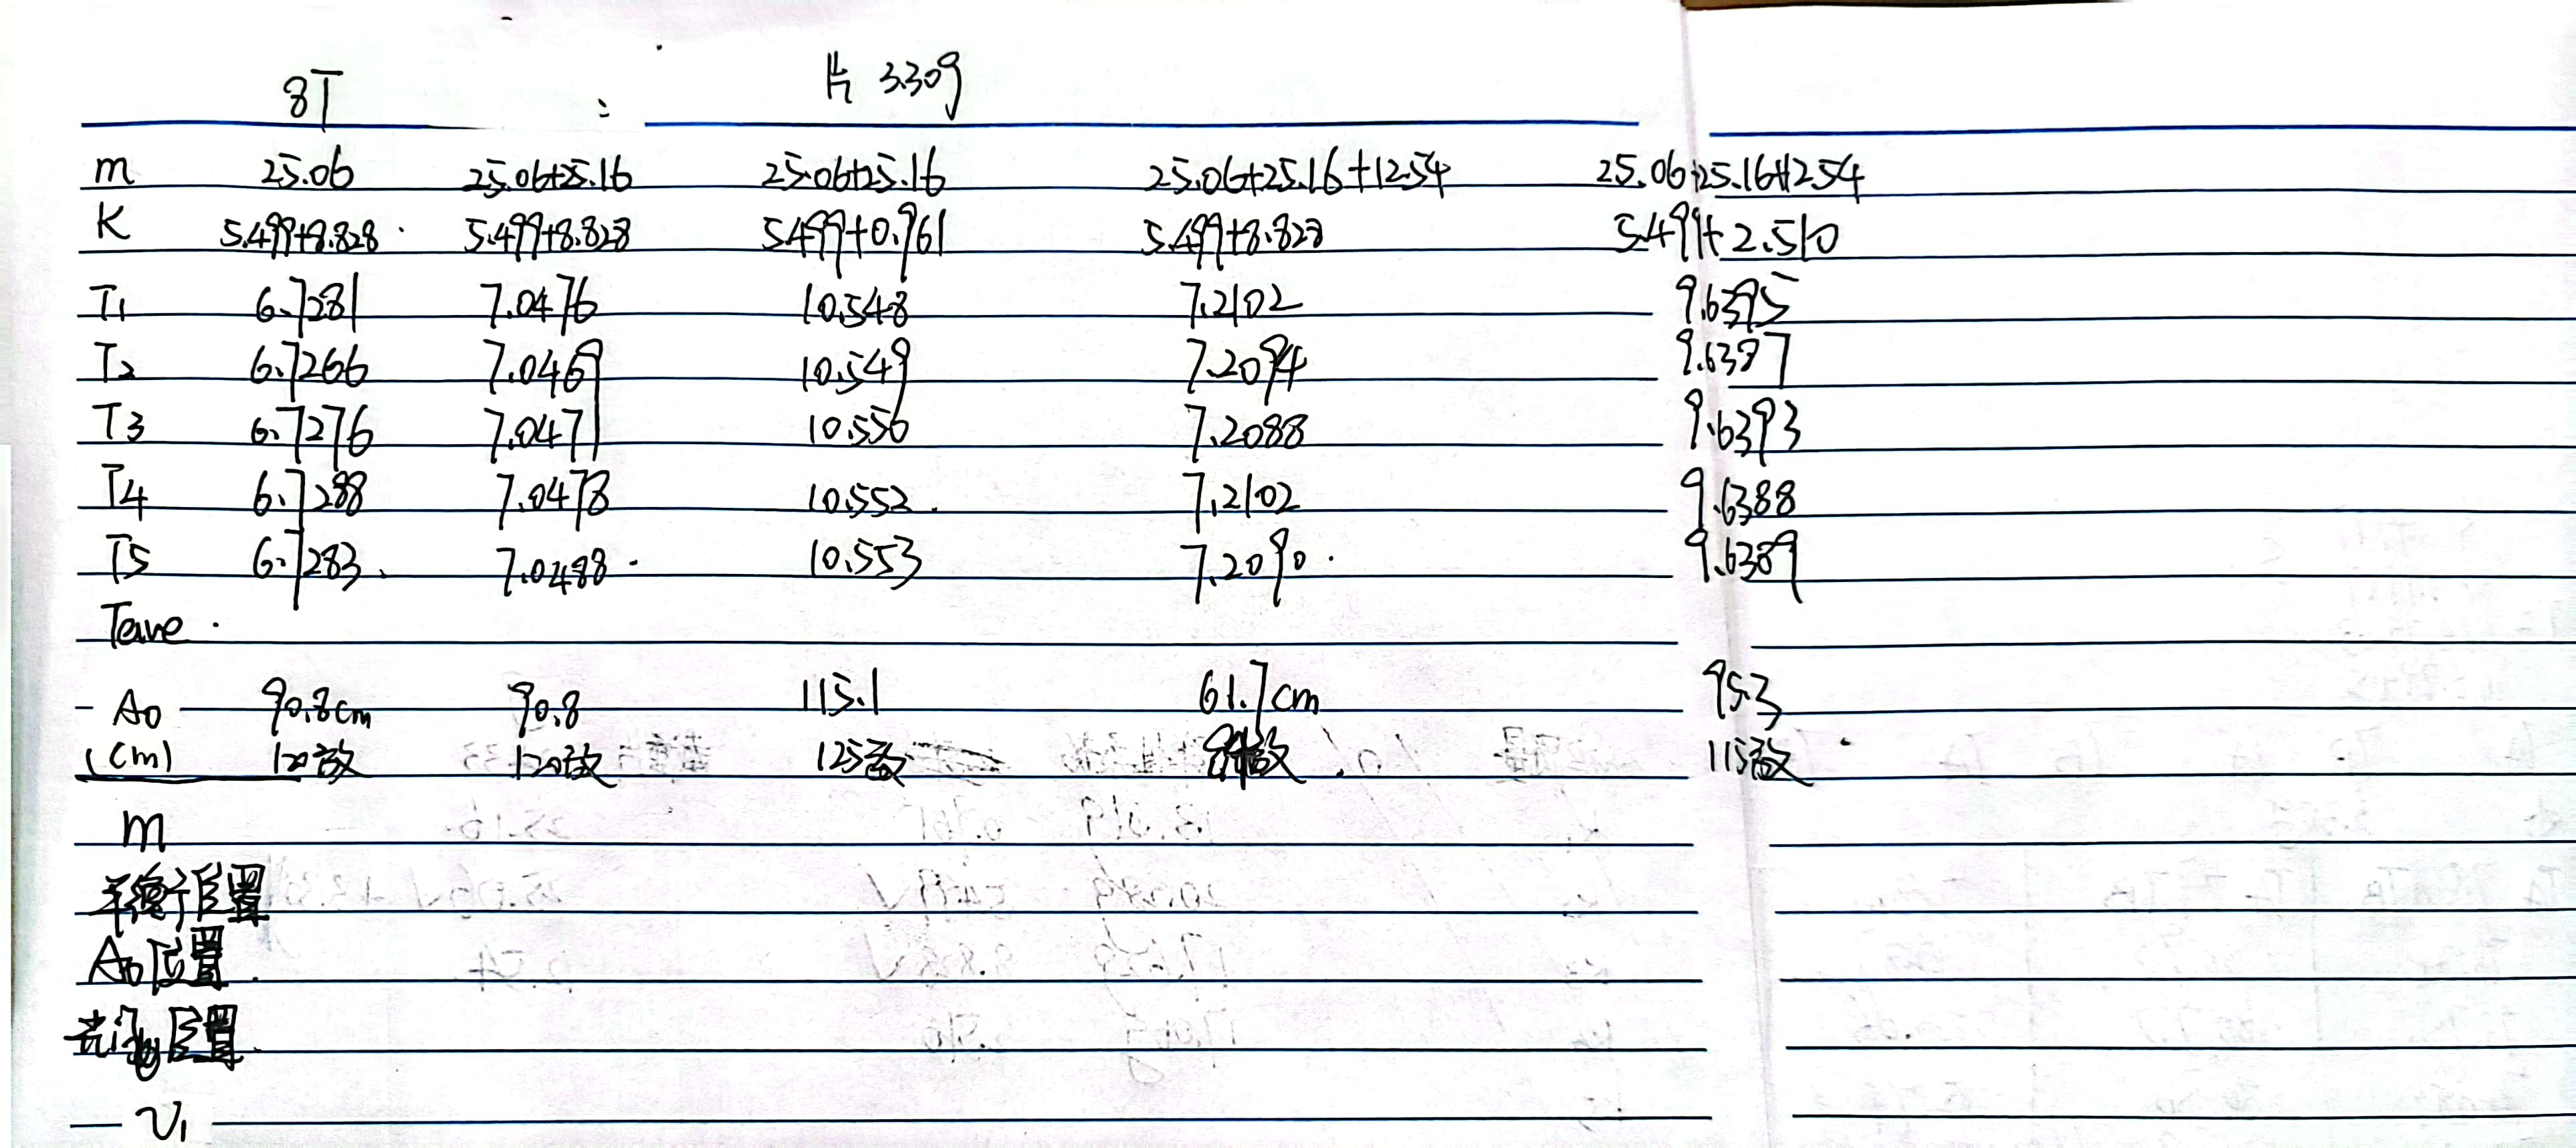
\includegraphics[width=1\textwidth]{yuanshishujv1.jpg}
  \caption{实验原理辅助用图}\label{yuanshishujv1}
\end{figure}
\newpage
%----------------------------------------------------------------------------
\begin{figure}[h]
  \centering
  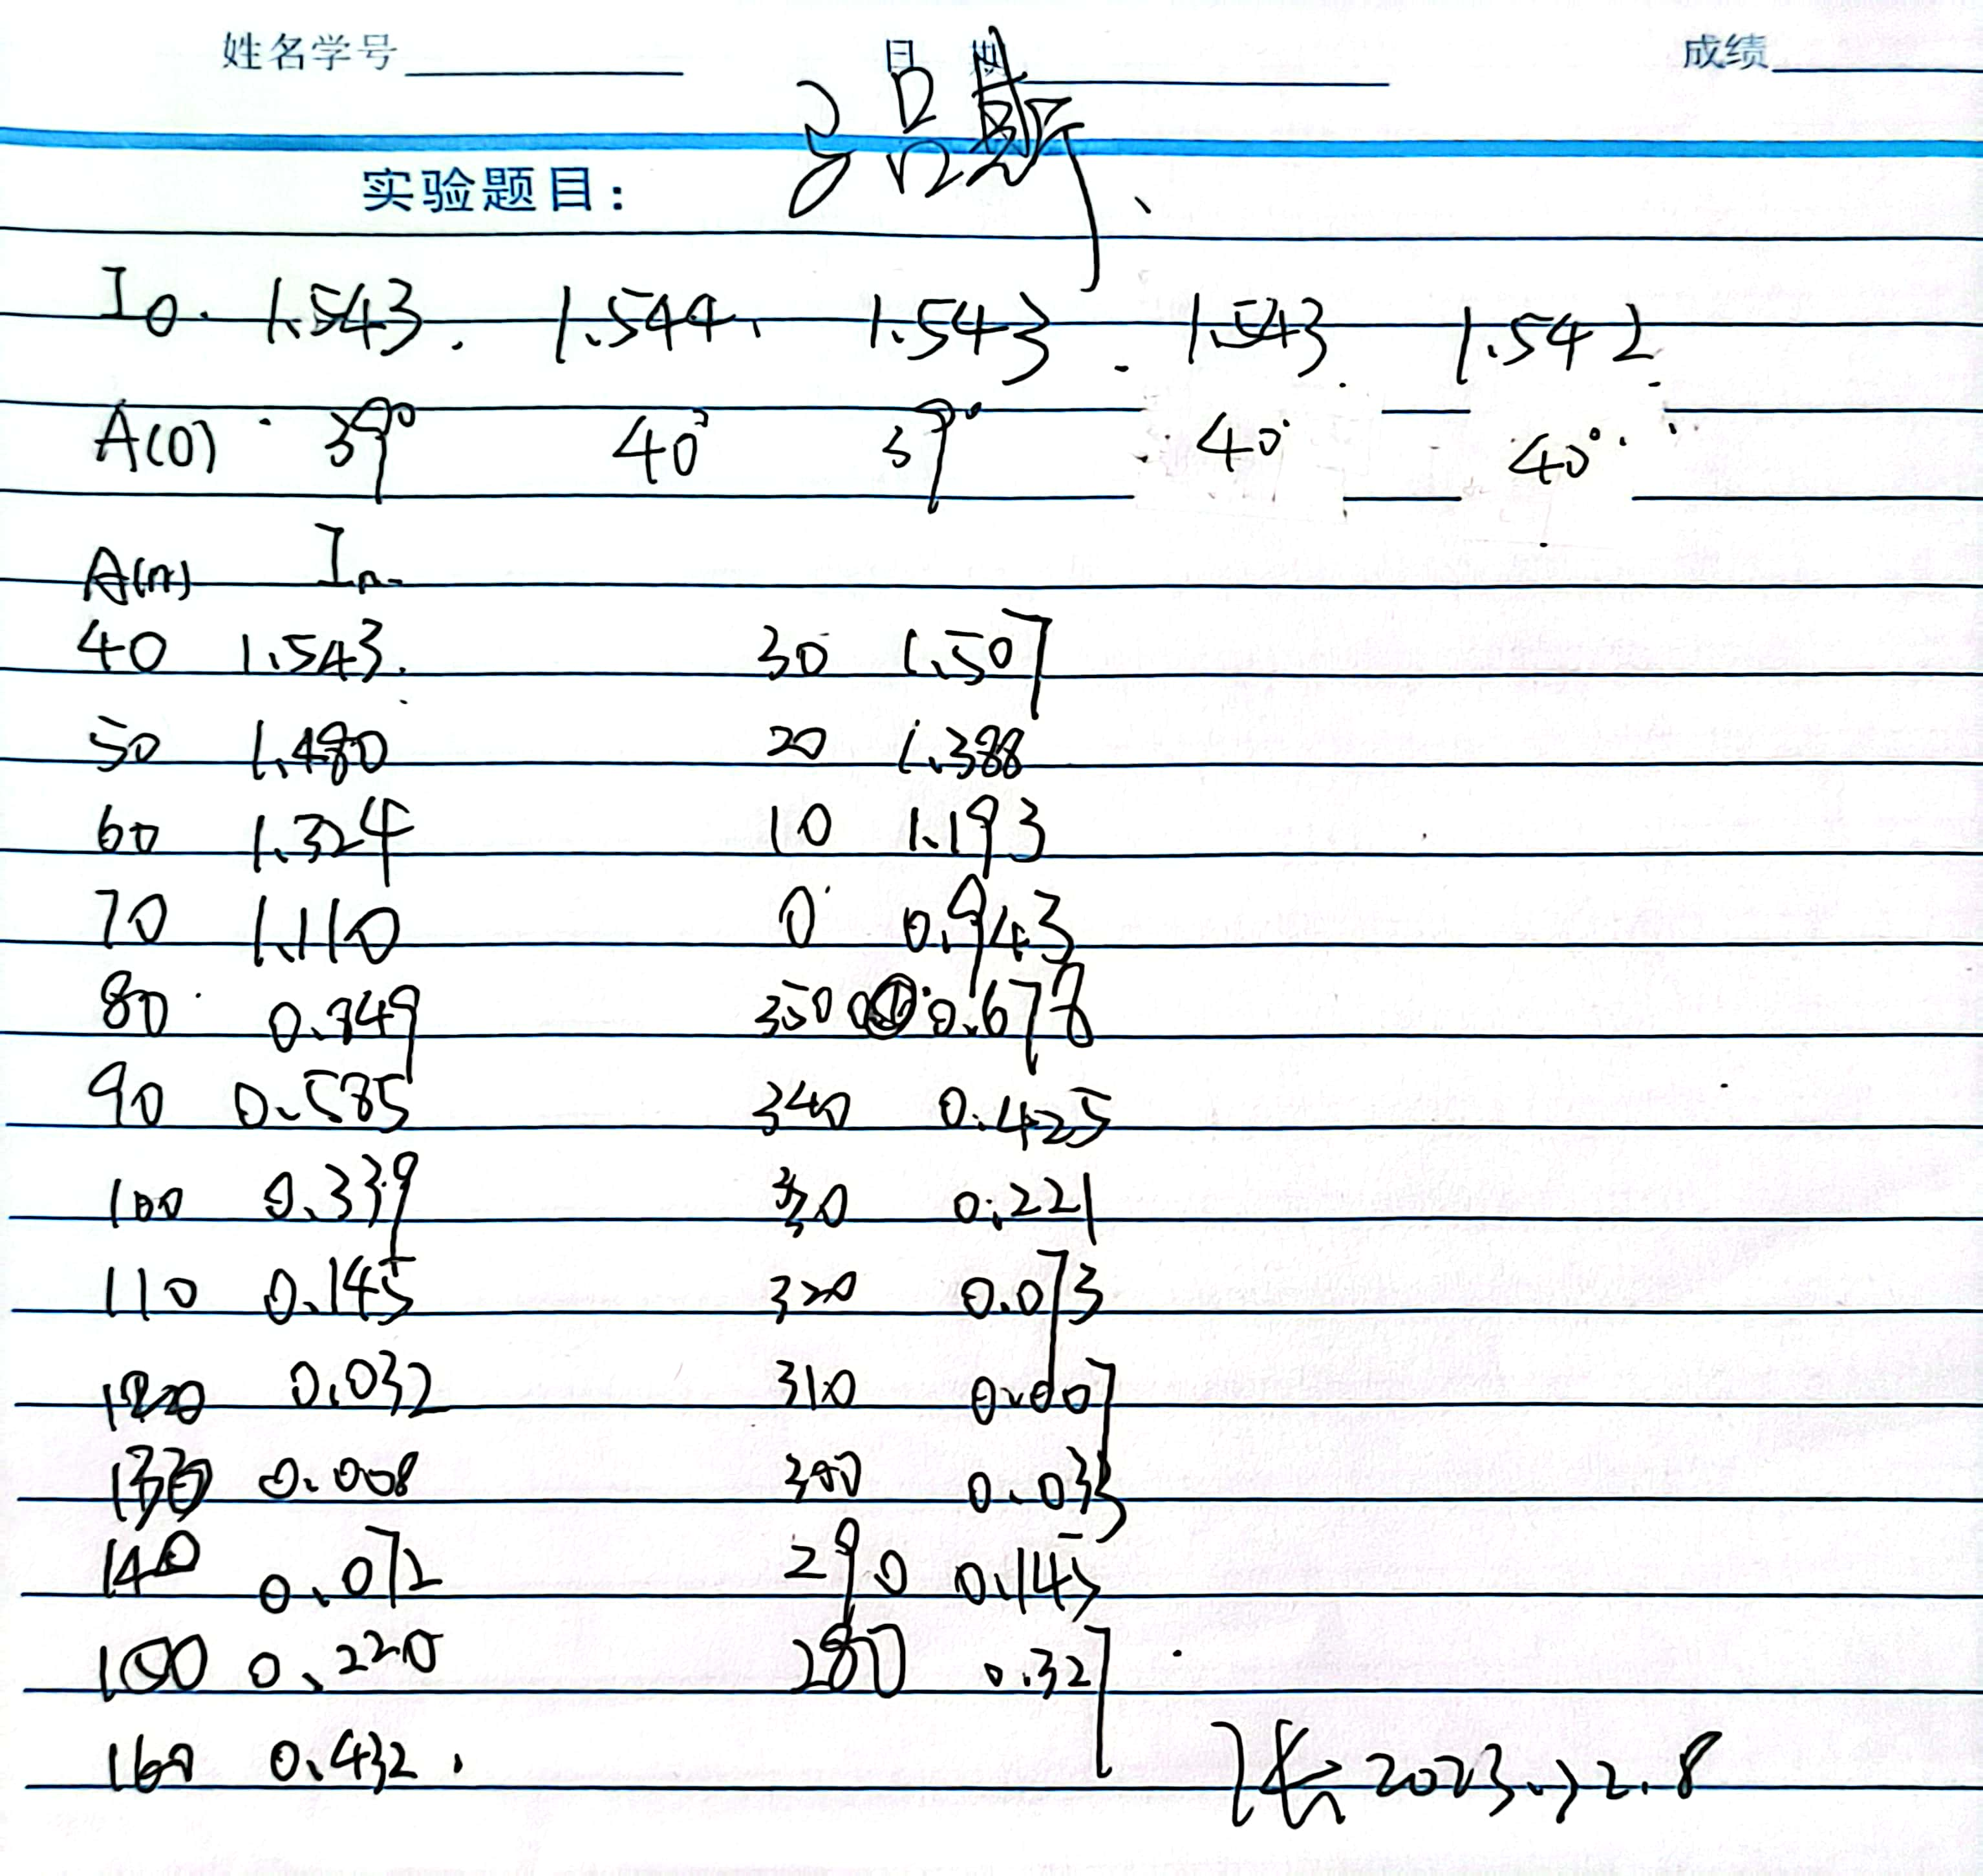
\includegraphics[height=1\textwidth,width=1\textwidth]{yuanshishujv2.jpg}
  \caption{实验原理辅助用图}\label{yuanshishujv2}
\end{figure}
\newpage
%----------------------------------------------------------------------------
\begin{figure}[h]
  \centering
  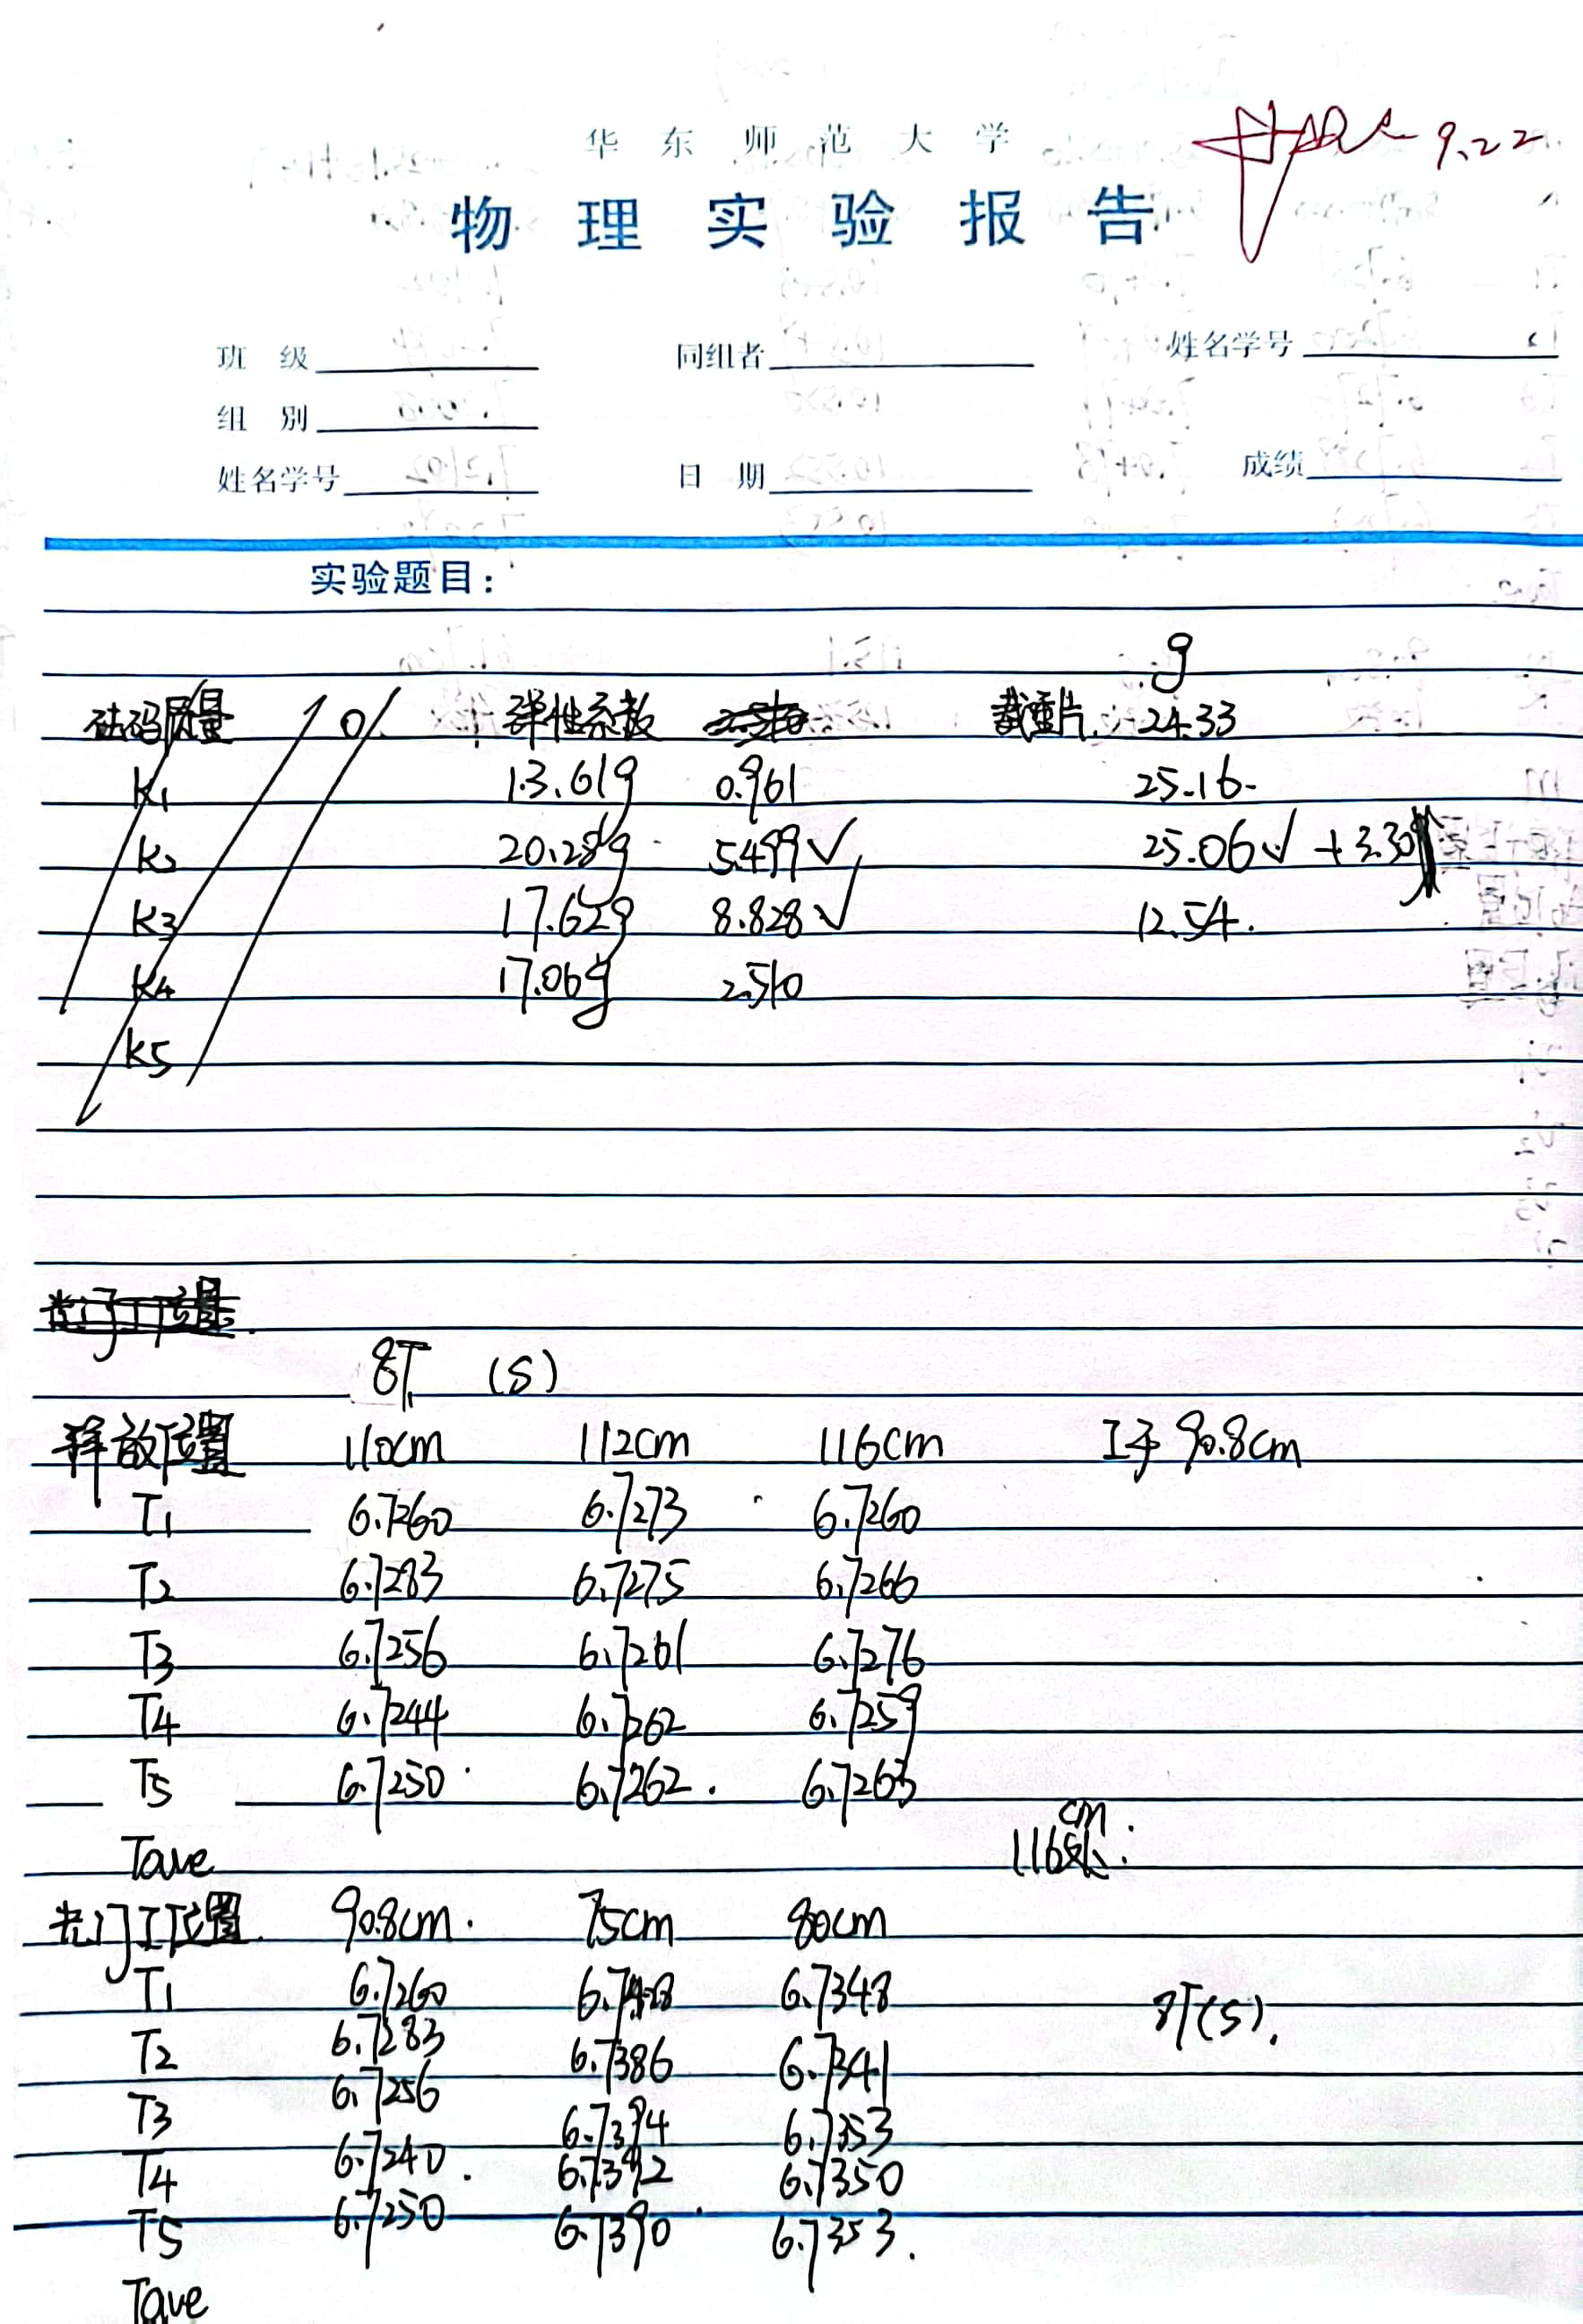
\includegraphics[height=1\textwidth,width=1\textwidth]{yuanshishujv3.jpg}
  \caption{实验原理辅助用图}\label{yuanshishujv3}
\end{figure}
\newpage

\section{实验数据处理}
弹簧质量显示如表\ref{tanhuangzhiliang}
\begin{table}[h]
  \centering   
  \caption{弹簧弹性系数及该系数弹簧的质量对应关系示意图}\label{tanhuangzhiliang}
  \begin{tabular}{| l || l |}
      \hline
      弹性系数的弹簧 & 弹簧质量(克)\\
      \hline
      0.961 & 13.61 \\
      \hline
      5.499 & 20.28 \\
      \hline
      8.828 & 17.62 \\
      \hline
      2.510 & 17.06 \\
      \hline                       
  \end{tabular}
\end{table}
  \subsection{验证位移方程}
  \begin{figure}[b]
    \centering
    \begin{minipage}[b]{0.48\textwidth}
      \centering
      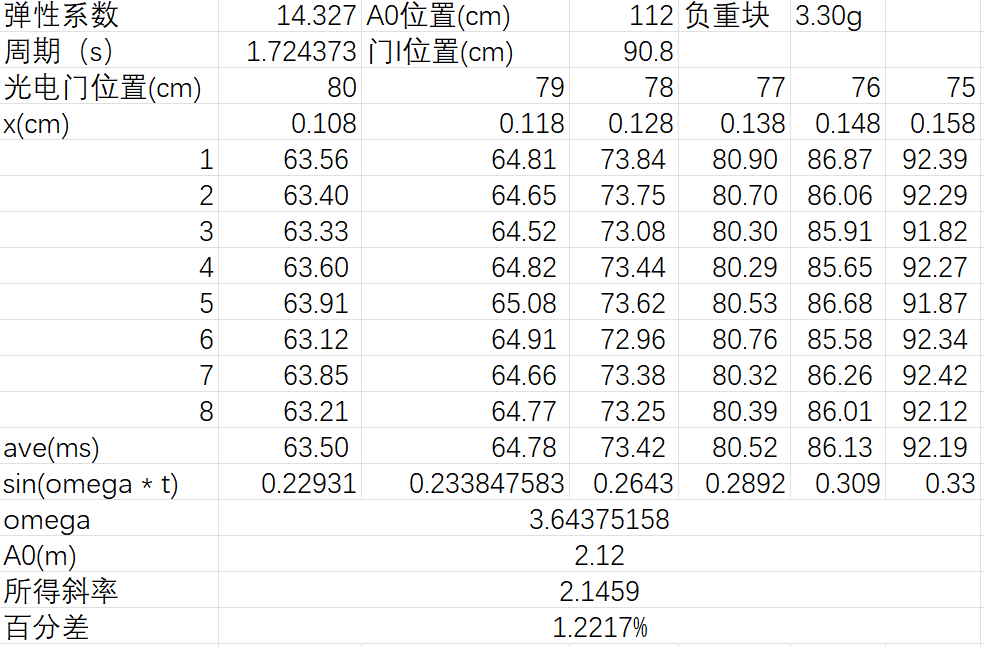
\includegraphics[width=0.46\textwidth]{yanzhengweiyifangchengshujv.png}
      \caption{验证位移方程数据}\label{yanzhengweiyifangchengshujv}
    \end{minipage}
    \begin{minipage}[b]{0.48\textwidth}
      \centering
      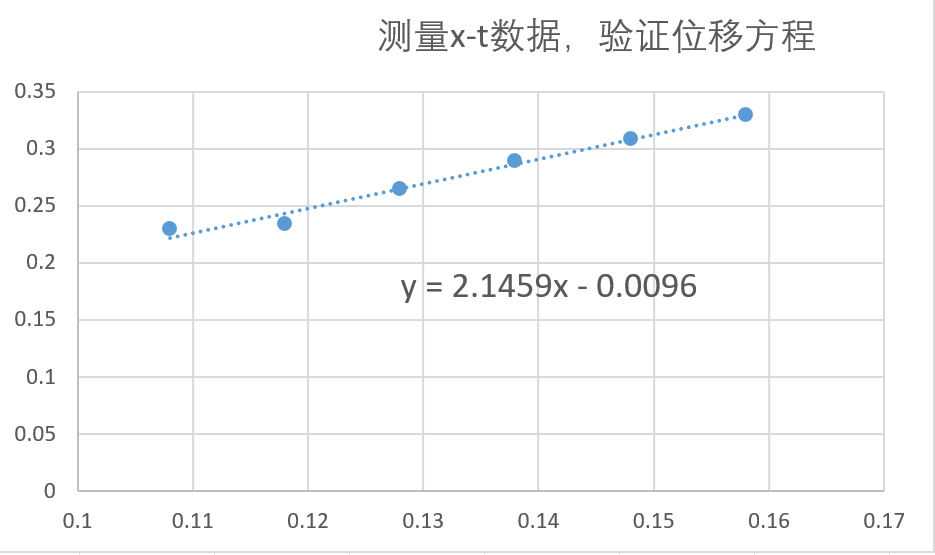
\includegraphics[width=0.46\textwidth]{yanzhengweiyifangchengzuotu.png}
      \caption{验证位移方程作图法}\label{yanzhengweiyifangchengzuotu}
    \end{minipage}
  \end{figure}

  实验数据处理如图\ref{yanzhengweiyifangchengshujv},其中计算可得实验理论$A_{0}=2.12dm$,而实验所得
  斜率,即实际测量的实际$A_{0}=2.1459dm$,两者的相差程度,即百分差为$1.2217\%$。可以证明位移方程
  $x=A\sin \left( \omega t + {\varphi}_{0} \right) \mbox{在}{\varphi}_{0} = 0 $时成立。

  实验中的误差可能来源于

  1、每次释放位置不能保证完全相同

  2、光电门传感器精度限制,以及挡光板的宽度

  3、实验中气垫滑轨不能保证完全水平,出现倾斜

  \subsection{验证振动周期与初始状态无关}
  \begin{figure}[t]
    \centering
    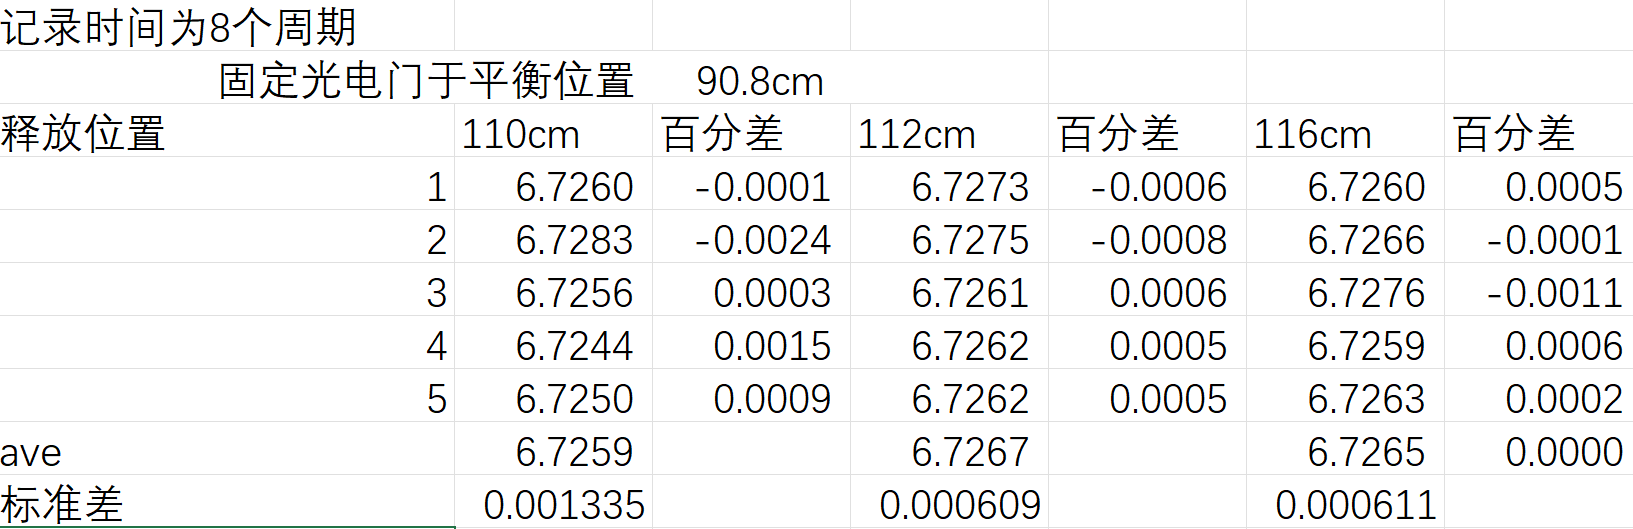
\includegraphics[height=0.3\textwidth,width=0.5\textwidth]{yanzhengwuguanshujv.png}
    \caption{验证振动周期与初始状态无关数据处理}\label{yanzhengwuguanshujv}
  \end{figure}
  验证振动周期与初始状态无关实验的数据及数据处理如图\ref{yanzhengwuguanshujv}所展示的那样。每个数据和该
  数据所在组平均值之间的相差不超过0.01s,除以八个周期后近似可以为相等,标准差也小于0.01。能验证振动周期与
  初始状态无关。

  实验中的误差可能来源于
  
  1、每次释放位置不能保证完全相同

  2、光电门传感器精度限制,以及挡光板的宽度

  3、实验中气垫滑轨不能保证完全水平,出现倾斜

  \subsection{验证周期公式$T=2\pi \sqrt{\frac{m}{k}}$}
  \begin{figure}[b]
    \centering
    \begin{minipage}[b]{0.48\textwidth}
      \centering
      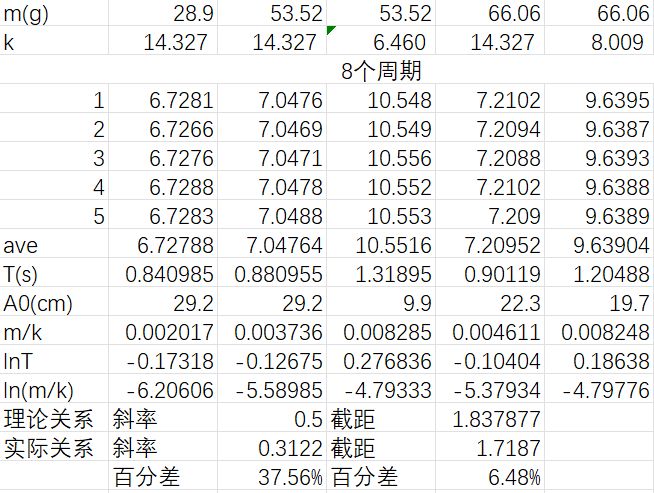
\includegraphics[width=0.46\textwidth]{yanzhengzhouqihanshu.png}
      \caption{验证周期公式$T=2\pi \sqrt{\frac{m}{k}}$实验数据}\label{yanzhengzhouqihanshu}
    \end{minipage}
    \begin{minipage}[b]{0.48\textwidth}
      \centering
      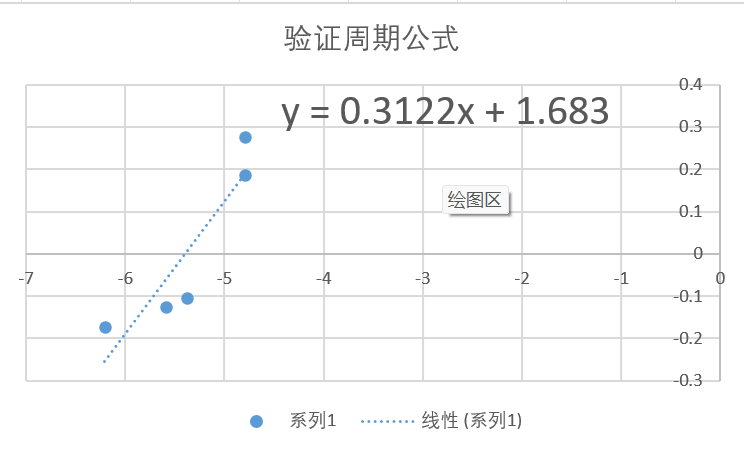
\includegraphics[width=0.46\textwidth]{yanzhengzhouqihanshuzuotu.png}
      \caption{验证周期公式$T=2\pi \sqrt{\frac{m}{k}}$数据处理}\label{yanzhengzhouqigongshizuotu}
    \end{minipage}
  \end{figure}
  验证周期公式的实验数据如图\ref{yanzhengzhouqihanshu}所示,实验数据处理如图\ref{yanzhengzhouqigongshizuotu}
  所示那样。本实验误差较大,涉及不确定度较多。
  实验中理论图像的斜率等于$\frac{1}{2}$,实验中理论截距为$\ln{2\pi}$。实际实验中图像的
  斜率等于$0.3122$,实际截距为$1.7187$。
  实验中理论和实际数据的百分差,斜率为$37.56\%$,截距为$6.48\%$

  实验中的误差可能来源于 
  
  1、每次释放位置不能保证完全相同

  2、光电门传感器精度限制,以及挡光板的宽度引入的误差。同时涉及质量称量,引入新的误差

  3、实验中气垫滑轨不能保证完全水平,出现倾斜

  实验中理论和实际的误差比较大,需要更多数据及更进一步的实验。其中斜率的误差较截距较大。
\newpage

\section{思考题}
  \subsection{频闪仪的作用}

  \subsection{确定弦线上的波节点的位置方法}

  \subsection{调节振动源的振幅大小对弦线振动产生的影响}
\newpage

\section{实验中个人的思考与感想}
  \subsection{对于实验个人观点}
  实验希望验证的内容时简谐振动的方程是否为简谐振动的方程。使用的方法时通过实验得到简谐振动的各种时间、振幅的数据,再代入方程中进行计算,是一种十分方便的验证方式。

  实验中采用的时气垫导轨的方式,通过气垫不断的喷气的设定,使滑块基本不与轨道摩擦,仅保留空气阻力作为阻碍。十分讨巧地避免了阻尼振动的问题。

  实验中使用的计时工具时光电门,通过仪器和线路的搭建,使用两个光电门获得各种时间数值。

  虽然实验的设计十分巧妙,避开了许多存在的问题,但是实验中依旧存在一些问题。在放置光电门的时候所在位置的读取存在误差,而且实验中通过光电门的速度虽然十分快,但是由于滑块上
  的挡光片的宽度难以消除,所以实验中还有些许多误差存在。实验中气垫导轨有时又由于气流不稳定等原因,存在在接往喷气机的一端风力较大,而另一端风力较小,存在\" 空气坡面\"的存在
  导致误差进一步加大。
  
  \subsection{实验中的总结}
  虽然实验设计十分巧妙,但是实际在应用中仍存在诸多问题。几个实验中多数数据较为准确误差也较小,但是也存在误差较大的数据导致最终和目标相差甚远。


\end{document}